% A workaround to allow relative paths in included subfiles
% that are to be compiled separately
% See https://tex.stackexchange.com/questions/153312/subfiles-inside-a-subfile-using-relative-paths
\providecommand{\main}{..}
\documentclass[\main/thesis.tex]{subfiles}
\externaldocument{previous}

\onlyinsubfile{\externaldocument{\main/tex/introduction}}

\SetKwProg{Fn}{Function}{}{} % add this line to solve the problem existing in algorithm

\begin{document}
\chapter{Link Prediction}
As we discussed in Section \ref{neighbor-based-metrics}, common-neighbors-based metrics are the simplest yet effective to predict missing links. They assume that two nodes are more likely to be connected if they have more common neighbors. Common neighbors (CN) is one of the most widespread measurements used in link prediction problem mainly due to its simplicity \cite{newman2001clustering}. Resource Allocation (RA) metric \cite{zhou2009predicting} is regarded as one of the best neighbor-based metrics because of its performance. Therefore, in this Chapter, we concentrate on CN and RA index.
\section{Link Prediction for Uncertain Graphs}
\subsection{Uncertain Version of Neighbor-based Metrics} \label{Uncertain-Version-of-Neighbor-based-Metrics}
To solve the problem of link prediction for uncertain graphs, one very naive/intuitive way is to regard the probability as a weight and apply weighted similarity metrics. However, there exists some problems. Figure \ref{problem-consider-probability-as-weight-link} is an example.

Nodes $\mathcal{V}_A$ and $\mathcal{V}_B$ are more likely to be connected than nodes $\mathcal{V}_D$ and $\mathcal{V}_E$ based on Equation \ref{WCN-previous}.
\begin{equation}
s_{AB} = 0.2 + 0.9 = 1.1
\end{equation}
\begin{equation}
s_{DE} = 0.5 + 0.5 = 1.0 < 1.1
\end{equation}

\begin{figure}
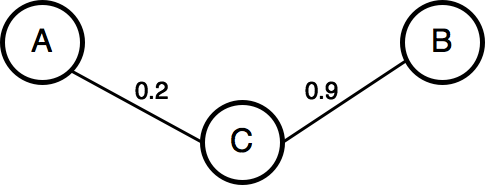
\includegraphics[scale = 0.3]{\main/img/common_neighbor_2.png}
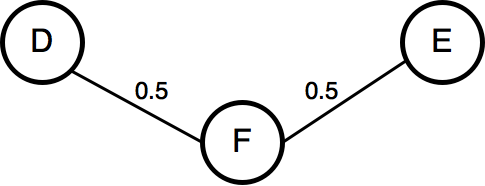
\includegraphics[scale = 0.3]{\main/img/common_neighbor_1.png}
\centering
\caption{An example showing the problem when considering the probability as a weight}
\label{problem-consider-probability-as-weight-link}
\end{figure}

However, because each edge may exist or not exist in the real world, both these two uncertain graphs have 4 possible worlds, as can be seen in Figure \ref{possible-world-link}.

\begin{figure}
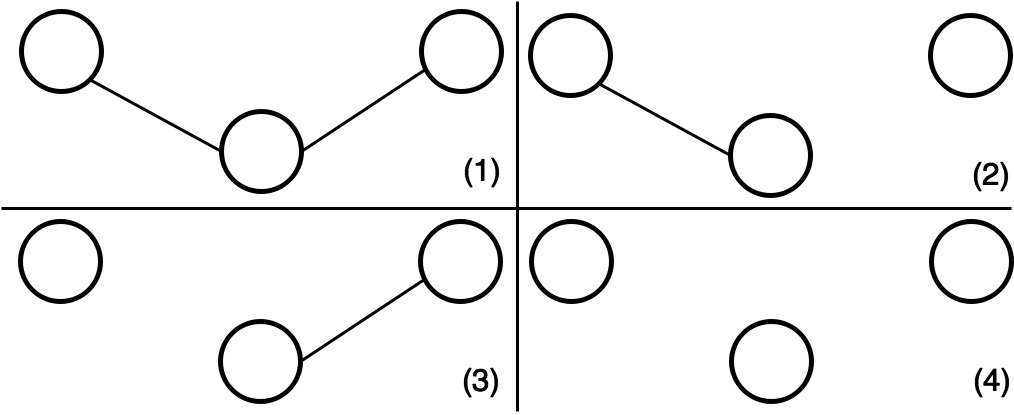
\includegraphics[scale = 0.3]{\main/img/possible_world.png}
\centering
\caption{Possible worlds}
\label{possible-world-link}
\end{figure}

Only when both edges $\mathcal{E}_{AC}$ and $\mathcal{E}_{BC}$ exist, node $\mathcal{V}_C$ is the common neighbor of nodes $\mathcal{V}_A$ and $\mathcal{V}_B$, as Figure \ref{possible-world-link}(1), the probability for this case is $0.2\times 0.9=0.18$. In this case, $s_{AB}=1$ based on Equation \ref{CN-previous}. If node $\mathcal{V}_C$ is not the common neighbor of nodes $\mathcal{V}_A$ and $\mathcal{V}_B$, as Figure \ref{possible-world-link}(2-4),  then $s_{AB}=0$. The probability for this case is 0.82. In comparison, the probability that $s_{DE}=1$ is $0.5\times 0.5=0.25$, while the probability of $s_{DE}=0$ is 0.75. Therefore, nodes $\mathcal{V}_D$ and $\mathcal{V}_E$ are more likely to be connected than nodes $\mathcal{V}_A$ and $\mathcal{V}_B$, because the probability of $s_{DE}=1$ is larger than $s_{AB}=1$. 

From this example, we can find that each uncertain edge in an uncertain graph may exist or not exist in a real world. If an uncertain graph has $|\mathcal{E}|$ uncertain edges, there will be $2^{|\mathcal{E}|}$ possible worlds in total, since each edge provides us with a binary sampling decision.

Given an uncertain network $\mathcal{G = (V,E,P)}$, we can sample each edge in $\mathcal{G}$ according to the probability $\mathcal{P}(e)$ to generate the possible graph $G = (V_G,E_G)$. We have $E_G \in \mathcal{E}$ and $V_G \in \mathcal{V}$. The probability $Pr(G)$ of sampling the possible graph is as follows:
\begin{equation}
Pr(G) = \prod_{e\in E_G}\mathcal{P}(e)\prod_{e\in \mathcal{E}, e\notin E_G}(1-\mathcal{P}(e))
\label{probability-of-possible-world}
\end{equation}
%\subsection{For uncertain networks}

For each possible world, its corresponding similarity measure may differ. When we calculate its similarity measures, we should take all possible worlds and their possibilities into account. Therefore, Common Neighbor and Resource Allocation in uncertain graphs can be represented as follows.

\textbf{Uncertain Common Neighbors (UCN)}
\begin{equation}
s_{xy}=\sum_{G\in \mathcal{G}}( Pr(G)\times|\Gamma_G(x)\cap\Gamma_G(y)|) \label{UCN-link}
\end{equation}
% \begin{equation}
% s_{xy}=\sum_{z\in \Gamma(x)\cap\Gamma(y)}p(x,z)\times p(y,z)
% \end{equation}

\textbf{Uncertain Resource Allocation (URA)}
\begin{equation}
s_{xy}=\sum_{G\in \mathcal{G}}( Pr(G)\times\sum_{z\in \Gamma_G(x)\cap\Gamma_G(y)}\frac{1}{k_G(z)}) \label{URA-link}
\end{equation}

Here, $\Gamma_G(x)$ denotes the set of neighbors of node $\mathcal{V}_x$ in the possible world $G$, $k_G(x)$ is the degree of node $\mathcal{V}_x$ in the possible world $G$.

\subsection{UCN Complexity Analysis} \label{CN-Complexity-Analysis}
We have a total of $2^{|\mathcal{E}|}$ possible worlds, and we can calculate CN value for each possible world in $O(k)$, where $k$ is nodes' average degree in the possible world. Therefore, the time complexity of calculating Common Neighbors value based on Equation \ref{UCN-link} is $O(2^{|\mathcal{E}|}k)$.

Assume $\Gamma_{xy} = \Gamma(x)\cap\Gamma(y)$ is the common neighbors set of nodes $\mathcal{V}_x$ and $\mathcal{V}_y$ in uncertain graph $\mathcal{G}$. Whether a node $\mathcal{V}_z \in \Gamma_{xy}$ is a common neighbor of nodes $\mathcal{V}_x$ and $\mathcal{V}_y$ in a possible world is independent of other nodes because it is determined by the existence of edges $\mathcal{E}_{xz}$ and $\mathcal{E}_{yz}$ in the possible world. Therefore, each node in $\Gamma_{xy}$ can be considered independently. If the existence probability over uncertain edges $\mathcal{E}_{xz}$ and $\mathcal{E}_{yz}$ are $\mathcal{P}_{x,z}$ and $\mathcal{P}_{y,z}$ respectively, only in $\mathcal{P}_{x,z}\times\mathcal{P}_{y,z}$ of all possible worlds, node $\mathcal{V}_z$ is the common neighbor of nodes $\mathcal{V}_x$ and $\mathcal{V}_y$. Therefore, Equation \ref{UCN-link} can also be represented as:
\begin{align*}
s_{xy}&=\sum_{G\in \mathcal{G}}( Pr(G)\times|\Gamma_G(x)\cap\Gamma_G(y)|)\\
&=\sum_{G\in \mathcal{G}}Pr(G)\sum_{z\in \Gamma(x)\cap\Gamma(y)}\mathbb{I}_{\Gamma_G(x)\cap\Gamma_G(y)}(z)\\
&=\sum_{z\in \Gamma(x)\cap\Gamma(y)}\sum_{G\in \mathcal{G}}Pr(G)\times\mathbb{I}_{\Gamma_G(x)\cap\Gamma_G(y)}(z)\\
&=\sum_{z\in \Gamma(x)\cap\Gamma(y)}\mathcal{P}_{x,z}\times\mathcal{P}_{y,z}
\end{align*}

When $z\in \Gamma_G(x)\cap\Gamma_G(y)$, $\mathbb{I}_{\Gamma_G(x)\cap\Gamma_G(y)}(z)=1$, otherwise, $\mathbb{I}_{\Gamma_G(x)\cap\Gamma_G(y)}(z)=0$.

By doing so, the time complexity for calculating $s_{xy}$ can be reduced to $O(K)$, where $K$ is nodes' average degree in the uncertain network.
%For each common neighbors in possible worlds, they are also common neighbors of two nodes in uncertain graphs. Therefore, each nodes of common neighbors in uncertain graph can be considered independently.
\subsection{URA Complexity Analysis}
We have a total of $2^{|\mathcal{E}|}$ possible worlds, and nodes' average degree in the possible world is $k$, then we can calculate RA value for each possible world in $O(k)$, so the time complexity of calculating Resource Allocation value based on Equation \ref{URA-link} is $O(2^{|\mathcal{E}|}k)$.
%(To calculate the RA value between node $x$ and node $y$, we only need consider edges connecting node $x$ and node $y$'s common neighbors. Assume the average degree of each node is $n$, then the number of edges connecting common neighbors is $mn$, so the time complexity can be reduced to $O(2^{mn}m)$.) \\

As mentioned in Section \ref{CN-Complexity-Analysis}, whether a node $\mathcal{V}_z \in \Gamma_{xy}$ is a common neighbor of nodes $\mathcal{V}_x$ and $\mathcal{V}_y$ in a possible world is independent of other nodes, besides, the number of edges each common neighbor owning is also independent of other nodes.  Therefore, each common neighbor can also be considered independently in this case. For the common neighbor node $\mathcal{V}_z$, when we generate possible worlds, we can only consider edges connecting to it, because the existence of other edges will not have an impact on $\mathbb{I}_{\Gamma_G(x)\cap\Gamma_G(y)}(z)$ and $k_G(z)$. Nodes' average degree in the uncertain network is $K$, so we can only consider $2^K$ possible worlds for the node $\mathcal{V}_z$, and the time complexity can be reduced to $O(2^{K}t)$, where $t=|\Gamma_G(x)\cap\Gamma_G(y)|$. 
\begin{align*}
s_{xy}&=\sum_{G\in \mathcal{G}}( Pr(G)\times\sum_{z\in \Gamma_G(x)\cap\Gamma_G(y)}\frac{1}{k_G(z)})\\
&=\sum_{z\in \Gamma(x)\cap\Gamma(y)}\sum_{G\in \mathcal{G}}Pr(G)\times\mathbb{I}_{\Gamma_G(x)\cap\Gamma_G(y)}(z)\times k_G(z)\\
&=\sum_{z\in \Gamma(x)\cap\Gamma(y)}\sum_{{G_z}\in \mathcal{G}_z}Pr({G_z})\times\mathbb{I}_{\Gamma_{G_z}(x)\cap\Gamma_{G_z}(y)}(z)\times k_{G_z}(z)\\
\end{align*}
$\mathcal{G}_z$ here stands for the uncertain sub-graph formed by edges connecting to node $\mathcal{V}_z$, and $G_z$ is the possible world based on the uncertain sub-graph $\mathcal{G}_z$.

\subsection{An efficient Algorithm for URA}

Only when both edges $\mathcal{E}_{xz}$ and $\mathcal{E}_{yz}$ exist, node $\mathcal{V}_z$ is the common neighbor of node $\mathcal{V}_x$ and node $\mathcal{V}_y$ in the possible world $G$, which means $\mathbb{I}_{\Gamma_G(x)\cap\Gamma_G(y)}(z)=1$. When node $\mathcal{V}_z$ is not the common neighbor of node $\mathcal{V}_x$ and node $\mathcal{V}_y$, $\mathbb{I}_{\Gamma_G(x)\cap\Gamma_G(y)}(z)=0$, it means those possible worlds will not have an impact on the value of $s_{xy}$. Edges $\mathcal{E}_{xz}$ and $\mathcal{E}_{yz}$ belong to the edge set which connects to node $\mathcal{V}_z$, so for those possible worlds which have an impact on the value of $s_{xy}$, node $\mathcal{V}_z$ at least has two edges $\mathcal{E}_{xz}$ and $\mathcal{E}_{yz}$.

Assume node $\mathcal{V}_z$ has $m$ extra edges in an uncertain graph except edges $\mathcal{E}_{xz}$ and $\mathcal{E}_{yz}$. Although it will result in $2^m$ possible worlds, the number of its edges in possible worlds will only range from 0 to $m$ (the number of edges node $\mathcal{V}_z$ has in total ranges from 2 to $m+2$), which means some of the possible worlds share the same number of edges. To calculate $s_{xy}$, one way is to iterate through all possible worlds, calculate each possible world's possibility based on Equation \ref{probability-of-possible-world} and its corresponding count of edges. The other way is to iterate through all the possible number of edges and calculate their corresponding probability, which can be seen as follows:
\begin{align*}
s_{xy}&=\sum_{z\in \Gamma(x)\cap\Gamma(y)}\sum_{{G_z}\in \mathcal{G}_z}Pr({G_z})\times\mathbb{I}_{\Gamma_{G_z}(x)\cap\Gamma_{G_z}(y)}(z)\times k_{G_z}(z)\\
&=\sum_{z\in \Gamma(x)\cap\Gamma(y)}\mathcal{P}_{x,z}\times\mathcal{P}_{y,z} \times \sum_{n=0}^{m}(P_{1\rightarrow m}^n \times \frac{1}{n+2})
\end{align*}

%For a common neighbor from $\Gamma_{xy}$, assume it has $m$ edges (except edges $\mathcal{E}_{xz}$ and $\mathcal{E}_{yz}$) in uncertain graph, though it will result in $2^m$ possible worlds, the number of its edges in possible worlds will only range from 0 to $m$, which means some of the possible worlds share the same number of edges. To calculate $\mathcal{R}$, one way is to calculate each possible world's possibility based on equation (7) and its corresponding counts of edges, the other way is to calculate the probability of having each possible number of edges.\\

% $\mathcal{K} = \{k_{G_{B-\mathcal{E}_{xz}-\mathcal{E}_{yz}}}|G_{B-\mathcal{E}_{xz}-\mathcal{E}_{yz}}\in \mathcal{G}_{B-\mathcal{E}_{xz}-\mathcal{E}_{yz}}\}$\\
% \begin{align*}
% \mathcal{R}&=\sum_{G_{B-\mathcal{E}_{xz}-\mathcal{E}_{yz}}\in \mathcal{G}_{B-\mathcal{E}_{xz}-\mathcal{E}_{yz}}}(Pr(G_{B-\mathcal{E}_{xz}-\mathcal{E}_{yz}})\times \frac{1}{k_{G_{B-\mathcal{E}_{xz}-\mathcal{E}_{yz}}}(z)+2})\\
% &=\sum_{n\in \mathcal{K}} (Pr(k_{G_{B-\mathcal{E}_{xz}-\mathcal{E}_{yz}}}(z)=n)\times \frac{1}{n+2})\\
% &=\sum_{n=0}^{m}P_m^n \times \frac{1}{n+2}
% \end{align*}

% \begin{align*}
% \mathcal{R}&=\sum_{G_{B-\mathcal{E}_{xz}-\mathcal{E}_{yz}}\in \mathcal{G}_{B-\mathcal{E}_{xz}-\mathcal{E}_{yz}}}(Pr(G_{B-\mathcal{E}_{xz}-\mathcal{E}_{yz}})\times \frac{1}{k_{G_{B-\mathcal{E}_{xz}-\mathcal{E}_{yz}}}(z)+2})\\
% &=\sum_{n=0}^{m} (Pr(k_{G_{B-\mathcal{E}_{xz}-\mathcal{E}_{yz}}}(z)=n)\times \frac{1}{n+2})\\
% &=\sum_{n=0}^{m}P_{1\rightarrow m}^n \times \frac{1}{n+2}
% \end{align*}

For the common neighbor $\mathcal{V}_z$, assume there are $m$ edges connecting to it except edges $\mathcal{E}_{xz}$ and $\mathcal{E}_{yz}$, so we can index them from 1 to $m$. $P_{1\rightarrow m}^n$ here stands for from edges $e_1$ to $e_m$, the probability that exactly $n$ among them exist in possible worlds. For the node with $m$ edges in uncertain graph, the number of its edges in possible worlds will range from 0 to $m$, and in other words, we need to compute $P_{1\rightarrow m}^0, P_{1\rightarrow m}^1, ..., P_{1\rightarrow m}^m$. 
%We proposed an efficient way to compute them, which works like merge sort. Conceptually, it works as follows:\\

We propose an efficient way to compute them, which can be regarded as a divide and conquer algorithm. Conceptually, it works as follows:

1) Divide the probability list into $n$ sublists, each containing 1 element, and compute the probability of having and not having this item respectively.

2) Repeatedly merge sublists to compute probabilities for sublists with more than 1 element. Here is the equation for merging the left half sublist and the right half sublist.
% \begin{align*}
% P_m^n=\sum_{i=max(0,n-\lceil m/2 \rceil)}^{min(n,\lfloor m/2 \rfloor)}P_{\lfloor m/2 \rfloor}^i P_{\lceil m/2 \rceil}^{n-i}
% \end{align*}
\begin{equation}
P_{1\rightarrow m}^n=\sum_{i=max(0,n-\lceil m/2 \rceil)}^{min(n,\lfloor m/2 \rfloor)}P_{1\rightarrow{\lfloor m/2 \rfloor}}^i P_{{\lfloor m/2 \rfloor}+1\rightarrow m}^{n-i}
\label{divide-conquer-specific}
\end{equation}

It can be implemented recursively. The result probability list has the length of $m+1$ and $P_{1\rightarrow m}^0, P_{1\rightarrow m}^1, ..., P_{1\rightarrow m}^m$ are saved sequentially in the result probability list. The full algorithm description can be found in Algorithm \ref{kEdgeProbability}.

% \newcommand\tikzmark[1]{%
%   \tikz[remember picture,overlay]\node (#1) {};}

% \algdef{SE}[FUNCTION]{Function}{EndFunction}%
%    [2]{\algorithmicfunction\ \textproc{#1}\ifthenelse{\equal{#2}{}}{}{(#2)}\vskip3pt}%
%    {\algorithmicend\ \algorithmicfunction}

% \newlength\funcwd
% \settowidth\funcwd{\algorithmicfunction}
% \addtolength\funcwd{3pt}

% \newcommand\Drawbox[3]{%
% \begin{tikzpicture}[remember picture,overlay]
% \coordinate (s#1) at ([xshift=-\funcwd,yshift=6pt]#1.north west);
% \coordinate (e#1) at ([xshift=#3,yshift=1pt]#2.south east);
% \draw (s#1) rectangle (e#1);
% \draw ([yshift=-1.2\baselineskip]s#1) -- ([yshift=-1.2\baselineskip]e#1|-s#1);
% \end{tikzpicture}
% }

% \begin{algorithmic}
% \Function{\tikzmark{start1}CallA}{$a$} \label{alg:a}
%     \State \Call{CalcSquare}{$a$}
% \Function{\tikzmark{start2}CalcSquare}{$b$} \label{alg:b}
%     \State \Return $b\times b$
% \EndFunction\tikzmark{end2}
% \EndFunction\tikzmark{end1}
% \end{algorithmic}

% \Drawbox{start1}{end1}{74pt}
% \Drawbox{start2}{end2}{55pt}


\begin{algorithm}
\KwData{Probability List $uncertainEdgeList$}
\KwResult{The probability list $probList$ of existing $n$ among $m$ edges, $n\in [0,m]$}
$uncertainEdgeListLength \leftarrow len(uncertainEdgeList)$\;
return $kEdge(0, uncertainEdgeListLength-1)$\;
// Inner Function\;
\Fn{kEdge(i, j)}{
 $length\leftarrow j-i+1$\;
 \eIf{$length=1$}{return $[1-uncertainEdgeList[i], uncertainEdgeList[i]]$}
 {
 $leftLength\leftarrow length // 2$\;
 $rightLength\leftarrow length - leftLength$\;
 // Divide Phase\;
 $left\leftarrow kEdge(i, i+leftLength-1)$\;
 $right \leftarrow kEdge(i+leftLength, j)$\;
 $probList \leftarrow [0] \times (length+1)$\;
 \For{each $n \in [0, length]$}{
	 \For{each $k \in [0, n]$}{
     	\If{$k<=leftLength$ and $n-k<=rightLength$}{
        	// Merge Phase\;
        	$probList[n] \leftarrow probList[n] + left[k]\times right[n-k]$\;
		}
 	}
 }
 return $probList$\;
 }
}
\caption{kEdgeProbability}
\label{kEdgeProbability}
\end{algorithm}

Based on the description of Algorithm \ref{kEdgeProbability}, we can find that $T(m)=2\times T(\frac{1}{2}m)+(1+2+...+m)$, so the time complexity of Algorithm \ref{kEdgeProbability} is $O(m^2)$. After calculating the probability list, we can easily calculate node $\mathcal{V}_z$'s contribution for $s_{xy}$.%To calculate $s_{xy}$, we can perform Algorithm 1 for each common neighbor of node $\mathcal{V}_x$ and $\mathcal{V}_y$, so the time complexity of computing $s_{xy}$ is $O(m^2t)$. The full algorithm to calculate $s_{xy}$ can be found in Algorithm 2.\\

It is reasonable to calculate $\mathcal{V}_z$'s contribution for $s_{xy}$ in $O(m^2)$. However, because the node $\mathcal{V}_z$ has $(m+2)$ neighbors in total, then any two of these neighbors (except those that are already connected, assume $u$ of them are already connected) will regard the node $\mathcal{V}_z$ as a common neighbor when calculating their similarity measures. Then node $\mathcal{V}_z$ will be calculated $(\frac{(m+2)(m+1)}{2}-u)$ times. 

%Each time we consider node $\mathcal{V}_z$, as mentioned in Algorithm 2, we pick out edges which are not connecting to the pair of nodes we are considering.\\

%of the pair of unconnected nodes we are considering
For each pair of unconnected nodes which have common neighbor $\mathcal{V}_z$, when we calculate node $\mathcal{V}_z$'s contribution on the similarity measure value, we firstly pick out edges which do not connect to the pair of nodes we are considering, then we apply Algorithm \ref{kEdgeProbability} to the list of these edges to get the probability list. For different pairs of unconnected nodes, the list of edges differ. To calculate $\mathcal{V}_z$'s contribution for one pair of nodes, the time complexity is $O(m^2)$. We have $(\frac{(m+2)(m+1)}{2}-u)$ pairs of unconnected nodes which have common neighbor $\mathcal{V}_z$, so the total time complexity will be $O(m^4)$.

This kind of time complexity is still very large. We can use the similar idea as we mentioned in Algorithm \ref{kEdgeProbability} to reduce the time complexity. In Algorithm \ref{kEdgeProbability}, we use the probability lists of the left half sublist and the right half list to compute the probability list of the full list. Actually, Equation \ref{divide-conquer-specific} has a more general form, which can be represented as follow:
\begin{equation}
P_{1\rightarrow m}^n=\sum_{i=max(0,n+k-m)}^{min(n,k)}P_{1\rightarrow k}^i P_{k+1\rightarrow m}^{n-i}
\label{divide-conquer-general}
\end{equation}
In Equation \ref{divide-conquer-specific}, we choose $k=\lfloor m/2 \rfloor$.

When we consider different pairs of unconnected nodes, node $\mathcal{V}_z$'s total edges remain the same, what differs is the set of two edges which connects to the pair of nodes we are considering, and it results in the difference of the remaining edges list which will be used in Algorithm \ref{kEdgeProbability}. To reduce the time complexity, the idea is to calculate the full edges list's corresponding probability list, which can be represented as $A = [P_{1\rightarrow m+2}^0, P_{1\rightarrow m+2}^1, ..., P_{1\rightarrow m+2}^{m+2}]$. For each pair of unconnected nodes, we want to calculate the remaining edges list's corresponding probability list, which can be represented as $B = [P_{1\rightarrow m}^0, P_{1\rightarrow m}^1, ..., P_{1\rightarrow m}^{m}]$. We can firstly find the two edges connecting to the pair of unconnected nodes, and calculate these two edges' corresponding probability list, which can be represented as $C = [P_{m+1\rightarrow m+2}^0, P_{m+1\rightarrow m+2}^1, P_{m+1\rightarrow m+2}^2]$. Then we can use $A$ and $C$ to calculate $B$ based on the Equation \ref{divide-conquer-general}. The full equations can be represented as follows:

\begin{align*}
\left\{
\begin{aligned}
P_{m+1\rightarrow m+2}^2 P_{1\rightarrow m}^{m} = P_{1\rightarrow m+2}^{m+2}\\
P_{m+1\rightarrow m+2}^1 P_{1\rightarrow m}^{m} + P_{m+1\rightarrow m+2}^2 P_{1\rightarrow m}^{m-1} = P_{1\rightarrow m+2}^{m+1}\\
P_{m+1\rightarrow m+2}^0 P_{1\rightarrow m}^{m} + P_{m+1\rightarrow m+2}^1 P_{1\rightarrow m}^{m-1} + P_{m+1\rightarrow m+2}^2 P_{1\rightarrow m}^{m-2} = P_{1\rightarrow m+2}^{m}\\
P_{m+1\rightarrow m+2}^0 P_{1\rightarrow m}^{m-1} + P_{m+1\rightarrow m+2}^1 P_{1\rightarrow m}^{m-2} + P_{m+1\rightarrow m+2}^2 P_{1\rightarrow m}^{m-3} = P_{1\rightarrow m+2}^{m-1}\\
...\\
P_{m+1\rightarrow m+2}^0 P_{1\rightarrow m}^{3} + P_{m+1\rightarrow m+2}^1 P_{1\rightarrow m}^{2} + P_{m+1\rightarrow m+2}^2 P_{1\rightarrow m}^{1} = P_{1\rightarrow m+2}^3\\
P_{m+1\rightarrow m+2}^0 P_{1\rightarrow m}^{2} + P_{m+1\rightarrow m+2}^1 P_{1\rightarrow m}^{1} + P_{m+1\rightarrow m+2}^2 P_{1\rightarrow m}^{0} = P_{1\rightarrow m+2}^2\\
\end{aligned}
\right.
\end{align*}

These equations are easy to solve, after we get $A$ and $C$, we can calculate probability list $[P_{1\rightarrow m}^0, P_{1\rightarrow m}^1, ..., P_{1\rightarrow m}^{m}]$ in $O(m)$. Though it takes $O(m^2)$ time to calculate $A$, when we consider different pairs of unconnected nodes which have common neighbor $\mathcal{V}_z$, $A$ only needs to be calculated once. To calculate different pairs of unconnected nodes' corresponding probability list $B$, we can firstly calculate their probability $C$ in constant time, and then use $A$ and $C$ to calculate $B$ in $O(m)$. Because we have $(\frac{(m+2)(m+1)}{2}-u)$ pairs of unconnected nodes, the time complexity of calculating $A$ can be ignored. To calculate node $\mathcal{V}_z$'s contribution for all unconnected nodes which have common neighbor $\mathcal{V}_z$, the time complexity is $O(m^3)$, and the average time complexity of calculating node $\mathcal{V}_z$'s contribution for a certain pair of unconnected nodes will be $O(m)$. To calculate $s_{xy}$, we can calculate nodes $\mathcal{V}_x$ and $\mathcal{V}_y$'s each common neighbor's contribution for $s_{xy}$ in $O(m)$, because nodes $\mathcal{V}_x$ and $\mathcal{V}_y$ have $t$ common neighbors in total. The time complexity of computing $s_{xy}$ is $O(mt)$. The overall algorithm for calculating $s_{xy}$ can be found in Algorithm \ref{Resource-Allocation-Value-Calculation}. Before running Algorithm \ref{Resource-Allocation-Value-Calculation}, we need to do the initialization step, which is described in Algorithm \ref{Initialization}. In Algorithm \ref{Initialization}, we iterate through all nodes in graph $\mathcal{G}$, calculate their probability lists $A$ and save them in a hash table. The hash table will be used in Algorithm \ref{Resource-Allocation-Value-Calculation}.

\begin{algorithm}
\KwData{An uncertain graph $\mathcal{G}$.}
\KwResult{Probability lists for all nodes in $\mathcal{G}$ saved in a hash table $dict$}
Hash table $dict \leftarrow \{\}$\;
\For{each node $\mathcal{V}_z \in \mathcal{G}$}{
Array $uncertainEdgeList \leftarrow$ all uncertain edges connecting to node $\mathcal{V}_z$\;
$dict[\mathcal{V}_z]\leftarrow kEdgeProbability(uncertainEdgeList)$\;
}
return $dict$\;
\caption{Initialization}
\label{Initialization}
\end{algorithm}

\begin{algorithm}
\KwData{Nodes $\mathcal{V}_x$, $\mathcal{V}_y$, an uncertain graph $\mathcal{G}$ and the hash table $dict$ after running Algorithm \ref{Initialization}}
\KwResult{Resource Allocation value for nodes $\mathcal{V}_x$ and $\mathcal{V}_y$ in $\mathcal{G}$}
$result \leftarrow 0$\;
\For{each node $\mathcal{V}_z \in \Gamma(x)\cap\Gamma(y)$}{
Array $uncertainEdgeList \leftarrow [ ]$\;
$probValue \leftarrow 1$\;
	\For{each node $\mathcal{V}_m$ connecting to node $\mathcal{V}_z$}{
    	\If{$\mathcal{V}_m=\mathcal{V}_x$ or $\mathcal{V}_m=\mathcal{V}_y$}{
        	$probValue \leftarrow probValue \times \mathcal{P}_{m,z}$\;
        	add $\mathcal{P}_{m,z}$ to $uncertainEdgeList$\;
        }
    }
    Array $probListC \leftarrow kEdgeProbability(uncertainEdgeList)$\;
    Array $probListA \leftarrow dict[\mathcal{V}_z]$\;
    Array $probListB \leftarrow $ use $probListA$ and $probListC$ to calculate $probListB$ based on the Equation \ref{divide-conquer-general}\;
    $oneNodeResult \leftarrow 0$\;
    \For{each $i \in [0,len(probListB))$}{
    	$oneNodeResult \leftarrow oneNodeResult + probListB[i] \times \frac{1}{i+2}$\;
    }
    $result \leftarrow result + probValue \times oneNodeResult$\;
}
return $result$\;
\caption{Resource Allocation Value Calculation}
\label{Resource-Allocation-Value-Calculation}
\end{algorithm}

\section{Experiments}
\subsection{Datasets}
\subsection*{Protein-Protein Interaction Network }
We used the protein-protein interaction network (PPI) created by Krogan \cite{krogan2006global}. Two proteins are linked if it is likely that they interact. The core network consists of 2708 proteins and 7123 interactions labeled with probabilities.

\subsection*{Enron Network}
We used the Enron dataset compiled by Shetty and Adibi \cite{shetty2004enron}. The dataset is a subset of Enron employees, comprised of emails sent between employees, resulting in a dataset with 50,572 emails among 151 employees. We used the same method as Section 5 in  \cite{pfeiffer2010probabilistic} to assign each edge with a possibility of occurrence. 

\subsection*{Synthetic Uncertain Network Based on Deterministic Network} \label{Synthetic-Uncertain-Network-Based-on-Deterministic-Network}
Since there are not many publicly available uncertain network datasets, we also generated an uncertain network based on a deterministic network. The dataset we used here is USAir. The US air transportation network contains 332 airports and 2126 airlines. Based on this network, we use the uncertain network generator  (Algorithm \ref{Uncertain-Network-Generator} as mentioned in Chapter \ref{generator-chapter}) to generate its corresponding uncertain network. In this experiment, the percentage of non-existential edges we choose to add is 20\%.

To test the prediction performance of an algorithm, the observed edges, $E$, are divided into two separate sets: training set $E^T$, is regarded as known information; and probe set $E^P$, is used for testing and no information therein is allowed to be used for prediction. Clearly, we have $E^T \cup E^P = E$ and $E^T \cap E^P = $\o. 

For protein-protein interaction network and synthetic uncertain network, we only know their connection information, so the training set $E^T$ and the probe set $E^P$ can be randomly divided. In this thesis, the training set $E^T$ and the probe set $E^P$ are assumed to contain 90\% and 10\% of the links respectively. To get more reliable result, each value is obtained by averaging over 100 independent runs of random division of training set and probe set.

Link prediction algorithms should be capable of detecting the dynamic relationships between members in a temporal social network. Because Enron dataset is time-evolving, the relations among social members change continuously over time, and links are constantly varying and evolving. Using link prediction algorithms, we can predict newly added links in future networks. In the experiment, we predict new communications between two employees in Enron Corporation after Dec. 5, 2000, based on historical data. The idea is that, if two employees have email records before Dec. 5, 2000, we generate a potential edge between them. Then we assign these edges with a probability following the method described in  \cite{shetty2004enron}. The resulting probabilistic graph consists of 110 nodes and 388 edges, and this graph is regarded as the training set. The testing set is formed by taking in all the edges formed after Dec. 5, 2000. After discarding employees that have not appeared in the list of 110 employees, as well as the edges that have appeared both before and after Dec. 5, 2000, we obtained 574 ground-truth edges with 110 distinct employees.
%Link prediction algorithms should be capable of detecting dynamic relationships between members in a temporal social network. Because Enron dataset is time-evolving, the relations among social members change continuously over time, links are constantly varying and evolving. Using link prediction algorithms, we can predict newly added links in future networks. In the experiment, we predict new communications between two employees in Enron Corporation after (a certain time), based on historical data. The idea is that, if two employees have email records before (a certain time), we generate a potential edge between them. Then we assign these edges with a probability following the method described in  \cite{shetty2004enron}. (Specifically, ...) The resulting probabilistic graph consists of ... nodes and ... edges, and this graph is regarded as training set. The testing set is formed by taking in all edges formed (after a certain time). After discarding employees that have not appeared in the list of ... nodes, as well as the edges that have appeared both (from 2001 to 2004) and (from 2005 to 2009) (before ... and ...), we obtained ... ground-truth edges with ... distinct authors.
%Because relations among social members change continuously over time, links in real world social networks are constantly varying and evolving. New links may appear and existing links may vanish from the network. For example, email communications between friends, transactions between businesses, and partnerships between scientific researchers are changing over time. Therefore, link prediction algorithms should be capable of detecting dynamic relationships between members in a temporal social network.

To evaluate the performance of prediction algorithms, we apply a standard metric called Precision to quantify the accuracy of prediction, which focuses on top-ranked latent links. It is defined as $L_r/L$, where among top-$L$ candidate links, $L_r$ is the number of accurate predicted links actually appearing in the testing period.


\subsection{Results and Evaluation}
As the literature  \cite{lu2010link,lu2011link,liu2011link,tan2014link,zhu2016link} suggested, the top $L$ is set to 100 in our experiments. To evaluate our metrics, we compare the results computed by the uncertain version of graph proximity measures with weighted and unweighted ones. The name for these algorithms and their corresponding descriptions are shown in Table \ref{algorithm-list-link}.%In the task of link prediction for uncertain networks, we can (1) pay no attention to probabilities and use the original metrics; (2) regard probability as weight and use weighted common-neighbor-based metrics; (3) use our uncertain version of common-neighbor-based metrics.\\
% Use uncertain version of common-neighbor-based metrics.

\begin{table}[]
\centering
\caption{Algorithm List}
\label{algorithm-list-link}
\begin{tabular}{ccc}
\hline
Algorithm Name & Description                     \\ \hline
CN/RA      & Pay no attention to probabilities and use the original metrics.  \\
WCN/WRA       & Regard probability as weight and use weighted metrics.  \\
UCN/URA    & Use our uncertain version of graph proximity measures. \\ \hline
\end{tabular}
\end{table}

The prediction accuracy on the 3 networks are shown in Table \ref{experiment-result-link}.

\begin{table}[]
\centering
\caption{Results}
\label{experiment-result-link}
\begin{tabular}{c|c|c|c||c|c|c}
\hline
\multirow{2}{*}{Datasets} & \multicolumn{3}{c||}{Common Neighbor}              & \multicolumn{3}{c}{Resource Allocation} \\ \cline{2-7} 
                          & CN            & WCN             & UCN             & RA        & WRA      & URA               \\ \hline
PPI                       & 0.472         & 0.5045          & \textbf{0.5288} & 0.4123    & 0.45     & \textbf{0.5728}   \\ \hline
Enron                     & \textbf{0.53} & 0.51            & 0.51            & 0.43      & 0.35     & \textbf{0.51}     \\ \hline
Synthetic Network         & 0.586         & \textbf{0.5892} & 0.5764          & 0.5772    & 0.5832   & \textbf{0.5902}   \\ \hline
\end{tabular}
\end{table}

From Table \ref{experiment-result-link}, we can find observe that uncertain version of Resource Allocation metric can significantly outperform the original and weighted Resource Allocation metrics. This shows that in the task of link prediction with edge uncertainty, it is worthwhile to take every possible worlds into account.

Our uncertain version of Common Neighbor metric also shows competitive prediction accuracy, though it only outperforms weighted and original Common Neighbor metrics in PPI dataset. In the other two datasets, the results achieved by the uncertain version are very close to the best result achieved by the other two metrics.% We can still think our uncertain version of Common Neighbor metric is competitive.

\section{Conclusion}
In this Chapter, we propose an uncertain version of graph proximity measures for the link prediction problem in uncertain networks. We propose a new algorithm to reduce the time complexity of computing uncertain version of graph proximity measures. By taking all possible worlds into consideration, the performance of link predictions are improved compared with original and weighted proximity measures.

\end{document}